\chapter{Fabrication}
\section{Requirements}
The main aim of this project is to establish a fabrication process for microcavity mirrors of medium-high finesse. As the microcavity will be implemented in a praticle trapping experiment it is essential to ensure geometrical compatibility between cavity and particle trap.

\subsection{Cavity Length}\label{ChapCavityLength}
As discussed in \autoref{ChapSensingFactor}, the sensing factor is a quantity which determines how strong the presence of a glass particle influences the optical properties of the cavity. \autoref{EqSensingFactor} is inversely proportional to the length of the cavity which was explained through the fact that a smaller mode volume will cause the volume of the nano-scaled, particle inside of the cavity to become larger in comparison to the mode volume.\\
However, the cavity dimensions cannot be made arbitrarily small. At the minimum cavity length $L$, clipping losses of the trapping beam (see \autoref{Fig:FigBeamWidth}) need to be negligible. Clipping of the trapping beam would dramatically reduce its efficiency and cause scattering of energy into undesired modes. It would also heat up the cavity mirror.\\
\begin{figure}[H]
	\includesvg[scale=0.7]{source/trapping_beam_width}
	\caption{The figure shows a sketch of the trapping experiment. The green lines show the profile of the Gaussian mode. $z_{\si{T}}$ is the radius of the trapping beam (red). The trapping beam has an $\si{NA}$ of $0.8$. $z_{\si{m}}$ is the distance of the cavity mirror from the trapping beam's focus.}
	\label{Fig:FigBeamWidth}
\end{figure}
In the following discussion we will derive an analytical solution for the minimum cavity length given the trapping beams presence. Furthermore, the entire Gaussian mode cross section has to fit onto the mirror surface which dictates a minimum diameter $D$ for the mirrors. The problem ultimately boils down to minimizing $L$ while at the same time maximizing $D$ without intersecting with $z_{\si{T}}$.\\
To know the limit for the mirror diameter $D$ we first need the trapping beam radius $z_{\si{T}}$. From \autoref{Fig:FigBeamWidth} we see that this radius can be described by the following formula:
\begin{equation}\label{EqTrapRadius}
	z_{\si{T}}(x)=x\tan\alpha
\end{equation}
Next we need to describe the mirror diameter $D$ in relation to the Gaussian beam. The beam waist radius of a Gaussian beam is given by:
\begin{equation}
	w(z)=w_0\sqrt{1+\left(\frac{z}{z_{{\si{R}}}}\right)^2}
\end{equation}
where $z_{\si{R}}$ is the Rayleigh length. The Rayleigh length is given by the beam waist radius at the focus of the Gaussian beam and by its wavelength. We can now use this to determine $D$. Since the beam further diverges while coupling light out of the cavity the thickness of the mirror also needs to be considered.  The polymer layer which forms the mirror can be estimated to have a thickness of around $25\um$ and the glass cover slip where the mirror is fixed upon has a thickness of around $160\um$. The resulting thickness of both materials is summarized in the term $\delta$. The beam waist radius we are interested in is therefore $w(z_{\si{m}}+\delta)$. To get the diameter from the radius we normally would multiply by two. However, to make sure that the entire beam hits the mirror we use a factor $\rho = 5$ instead. The diameter is then defined by:
\begin{equation}\label{BeamDiameter}
	D(z_{\si{m}})=\rho\cdot w(z_{\si{m}}+\delta)
\end{equation}
Through simple algebra the mirror distance from the trapping beam focus is then given by:
\begin{equation}\label{EqMirrorDistance}
	z_{\si{m}}(D)=z_{\si{R}}\sqrt{\left(\frac{D}{\rho w_0}\right)^2-1}-\delta
\end{equation}
As stated at the beginning, we need to make $D$ as large as possible while keeping $z_{\si{m}}$ as small as possible. This requirement can be stated as follows:
\begin{equation}
	2\cdot z_{\si{T}}(x=D/2)=z_{\si{m}}(D)
\end{equation}
Note that we put a factor two in front of the trapping beam radius for safety reasons. If we plug \autoref{EqMirrorDistance} and \autoref{EqTrapRadius} into our requirement we get a quadratic equation which can be solved for $D$.
\begin{equation}
	D=\frac{-\delta\tan\alpha+\sqrt{\delta^2\tan^2\alpha -\left[\tan^2\alpha-\left(\frac{z_{\si{R}}}{\rho w_0}\right)^2\right]\left[\delta^2+z_{\si{R}}^2\right]}}{\tan^2\alpha-\left(\frac{z_{\si{R}}}{\rho w_0}\right)^2}
\end{equation}
Now we can estimate the cavity length $L=2\cdot z_{\si{m}}(D)+\delta$. To get actual numbers we have to fix the beam waist radius $w_0$ of the cavity mode at the focus. The estimated value for $w_0$ can range from $2\um$ to about $40\um$. In reality the focus width will be determined by the cavity dimensions themselves. To stay within the defined range of $w_0$ a cavity which has a length of $L\approx 500\um$ with mirrors of diameter $D\approx 200\um$ is a very robust choice.

\subsection{Wavefront radius}
For a Gaussian mode to resonate inside the cavity the wavefront radius of the beam has to match the curvature of the cavity mirror. Since we are using a hemispherical cavity, primarily for alignment reasons [ref], we have one mirror without curvature and one mirror which is spherical. The wavefront radius of the beam depends on the cavity length $L$.
\begin{equation}\label{EqWfRadius}
	R(L)=L\left[1+\left(\frac{z_{\si{R}}}{L}\right)^2\right]
\end{equation}
\begin{figure}[H]
	\includesvg[scale=0.7]{source/wf_radius}
	\caption{This figure shows the dependence of the wavefront radius $R$ of the Gaussian beam on the cavity length $L$ at a fixed $w_0$.}
\end{figure}
\autoref{EqWfRadius} does also depend on the Rayleigh length $z_{\si{R}}$.
\begin{equation}\label{EqRayleighRange}
	z_{\si{R}}=\frac{\pi w_0^2}{\lambda}
\end{equation}
While discussing the cavity length in the last section it was stated that the beam waist radius at the origin which also defines the wavefront radius through $z_{\si{R}}$, is determined by the cavity dimensions and has a certain allowed range. This is the reason why the $R$ does not have to be exact but can vary between $0.7\mm$ to $1.0\mm$. This is very important for process stability as we will see later on.
%\begin{equation}
%	R(w_0)=z_{\si{m}}\left[1+\frac{\pi^2w_0^4}{\lambda^2z_{\si{m}}^2}\right]
%\end{equation}

\subsection{Surface roughness}
The surface roughness of the cavity mirrors is of paramount importance while planning the fabrication of the microcavity mirrors. How the surface roughness influences the cavity losses is described by the following simple formula [ref]:
\begin{equation}
	L_{\si{sc}}=\left(\frac{4\pi\sigma_{\si{sc}}}{\lambda}\right)^2
\end{equation}
The finesse which defines what portion of the light remains inside of the cavity after one round trip is defined as [ref]:
\begin{equation}
	\mathcal{F}=\frac{2\pi}{L_{\si{sc}}}
\end{equation}
It can be seen that the finesse degrades substantially with an increasing surface roughness.
\begin{figure}[H]
	\includesvg[scale=0.7]{source/finesse_rms}
	\caption{It can be seen how the finesse of the cavity degrades as a function of the surface roughness (RMS). From a roughness of $0.5\si{nm}$ to $1.5\si{nm}$ the finesse has already degraded by one order of magnitude.}
\end{figure}
As explained in \autoref{ChapInformationRetrievalRate}, the linewidth of the cavity has to be large enough such that the particle motion can be followed without much delay. This means the finesse cannot be too high. However, the lowering of the finesse has to take place through the light leaving the cavity through one of the mirrors and not through scattering losses due to rough mirror surfaces. For this reason the aim is to fabricate mirrors with a roughness below $0.6\nm$ which corresponds to a scattering loss of less than $23.4\ppm$.
\newpage

\section{Process}
In the following section the fabrication process that was put together, based on extensive research with different fabrication approaches, will be described in detail.

\subsection{Overview}
The fabrication of the microcavity consists in the mainly in the manufacturing of a tiny spherical mirror. \autoref{Fig:fabrication_flowchart} shows schematically in what order the different steps of the fabrication process are arranged.
\begin{figure}[H]
	\includesvg[scale=0.3]{source/fabrication_flowchart}
	\caption{This flowchart shows schematically in which order the various fabrication steps are arranged.}
	\label{Fig:fabrication_flowchart}
\end{figure}
The process produces in the end a transparent shape of the mirror. In order for the mirror to fulfill its purpose it has to be coated with a reflective layer. This step is done by [company], an external company that specializes in coating sensitive structures on different scales.
\subsection{Cleaning}
The complete fabrication process takes quite some time to be completed. All steps combined up to the point where the mirror shape can be measured to determine its surface roughness, takes about twenty hours. To protect the mirrors from being contaminated while being fabricated, all fixtures and tools have to be clean. They are cleaned by putting them into a bath of acetone and then ultrasonicate them for roughly twenty minutes. After that the step is repeated with Isopropanol (longname) instead of acetone. Drying the components in an oven finalizes this step.
\subsection{Stamp fabrication}\label{ChapStampFabrication}
The fabrication of the stamps is one key step in the fabrication process. Fabricating the steps reliably is crucial to make the process stable. Various methods for creating stamps made from Siliciumdioxide exist. Some use pulsed lasers to melt them [ref]. Other methods use cylindrical holes to let spherical drops form inside while the whole setup is put into a high temperature oven [ref]. Our method uses a small blowtorch [ref] which can be bought regularly and a specially made machine which spins the glass medium while it is being melted. With the spinning it is ensured that the drop that the glass forms a symmetrical, spherical drop while being melted.\\
The material we use for this procedure are glass cylinders extracted from a standard multimode communication fiber of one millimeter thickness. To do this we use a special tool is used to remove the cladding. After that, we ultrasonicated the fiber piece in Acetone to remove the buffer layer. With this done the melting procedure can be initiated.
\begin{figure}[H]
	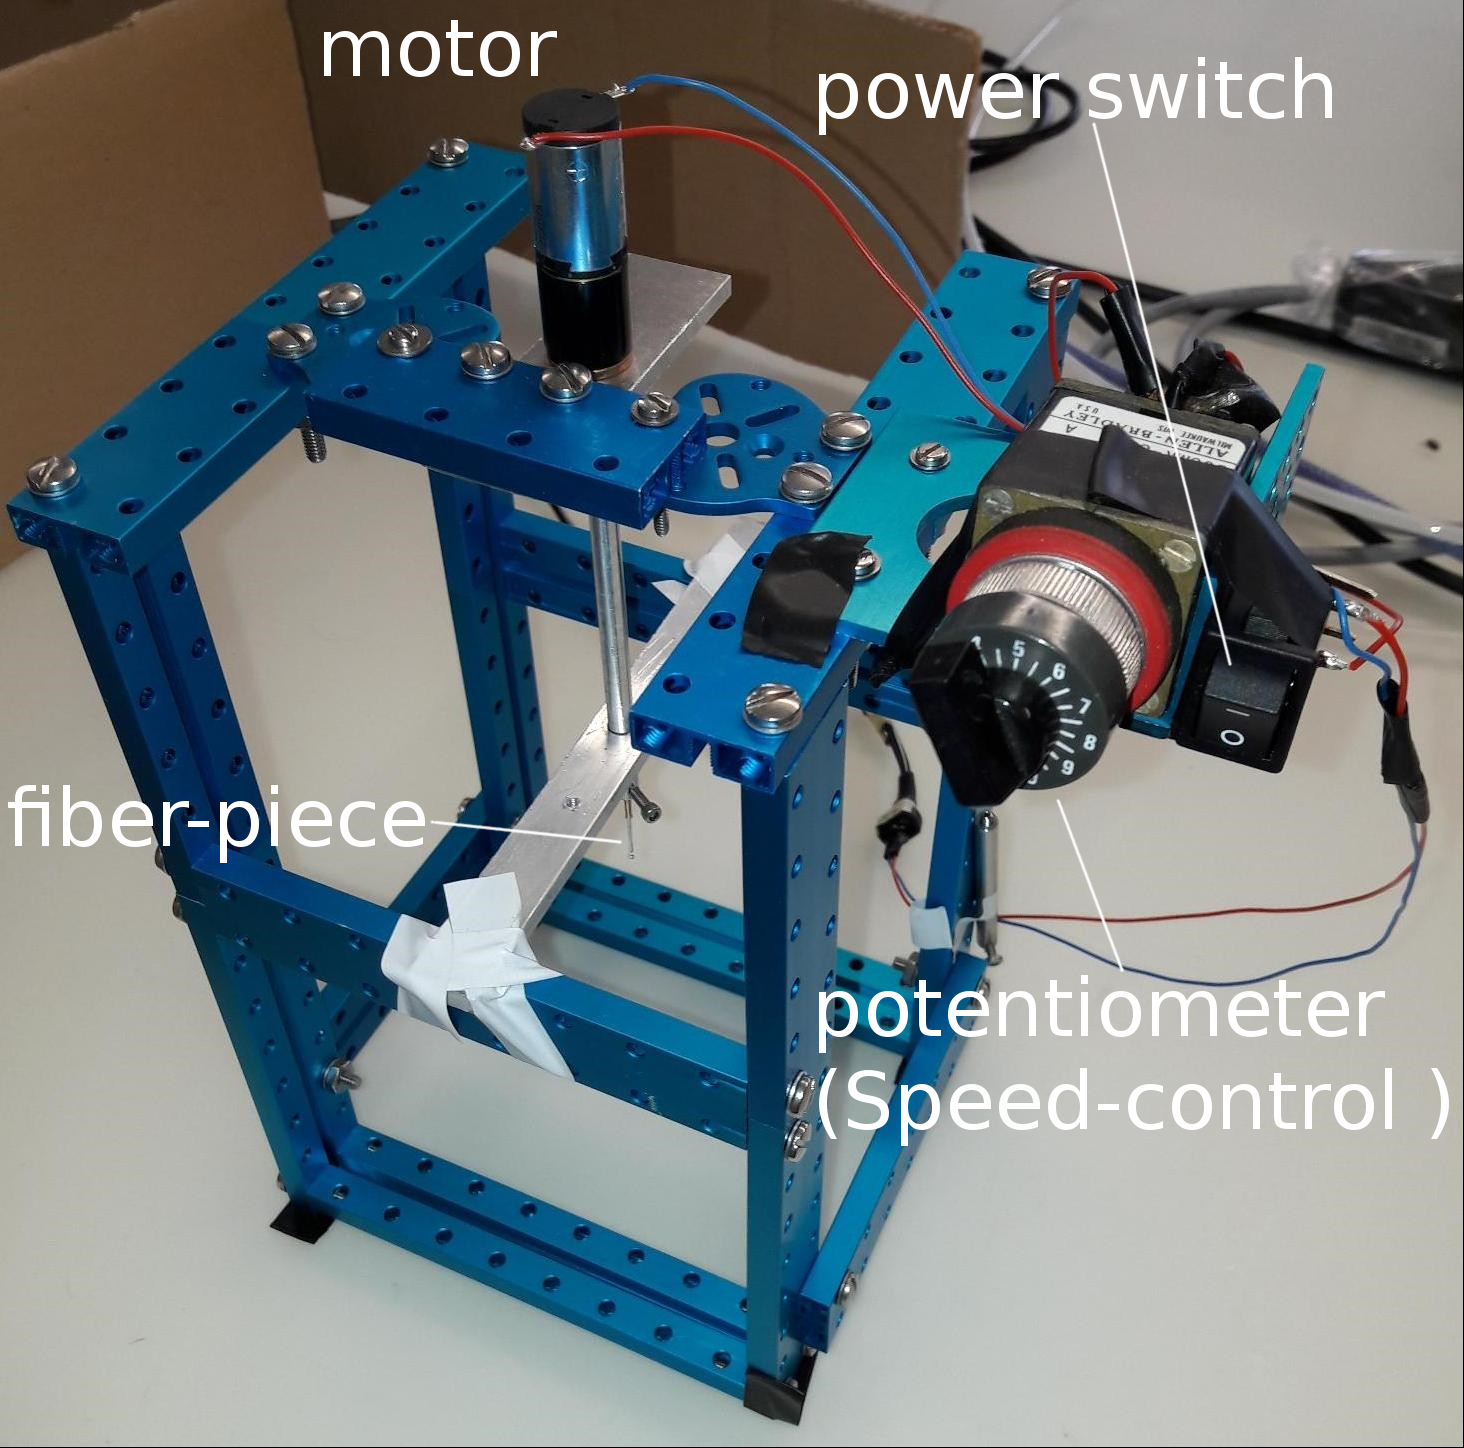
\includegraphics[scale=0.3]{source/melting_machine}
	\caption{A picture of the machine used for melting the glass rods. The framing is made from a construction kit from Makeblock. Some parts of the framing are custom made parts made from aluminum. The motor is from Maxxon (870 rpm, $41 \si{Nmm}$).}
	\label{Fig:Melting_machine}
\end{figure}
Without the spinning at approximately $11.4\si{Hz}$ (would be around $14.5\si{Hz}$ without the straightening fixture around the axles) the drop would not form a sphere in a controlled manner. \autoref{Fig:Melting_nonrotating} shows schematically how the formation without the spinning motion would look.
\begin{figure}[H]
	\includesvg[scale=0.3]{source/melting_nonrotating}
	\caption{Schematic depiction of a drop melted without the rotating motion during the process.}
	\label{Fig:Melting_nonrotating}
\end{figure}
With the machine shown in \autoref{Fig:Melting_machine} this problem can be omitted and the radius of the drop can be controlled by varying the speed of the machine and also by holding the blowtorch at different heights.
\begin{figure}[H]
	\includesvg[scale=0.3]{source/melting_rotating}
	\caption{Schematic depiction of the melting process with rotating axis.}
\end{figure}
For the actual melting we used two different process gases: Acetylene at a pressure of $0.4\si{bar}$ and Oxygen at a pressure of $0.2\si{bar}$. To prevent soot from contaminating the stamp it is important to add Oxygen to the Acetylene flame. If the yellow in the flame disappears and a blue glow is emitted from the center of the flame the blowtorch is set up properly. The melting then simply takes place by holding the flame of the blowtorch up to the rotating glass cylinder at approximately four millimetres above the lower end and waiting for the glass to melt and expand into a sphere. The blowtorch can then be turned off and in a short amount of time the glass cools down and forms a transparent sphere at the lower end of the cylinder.
\begin{figure}[H]
	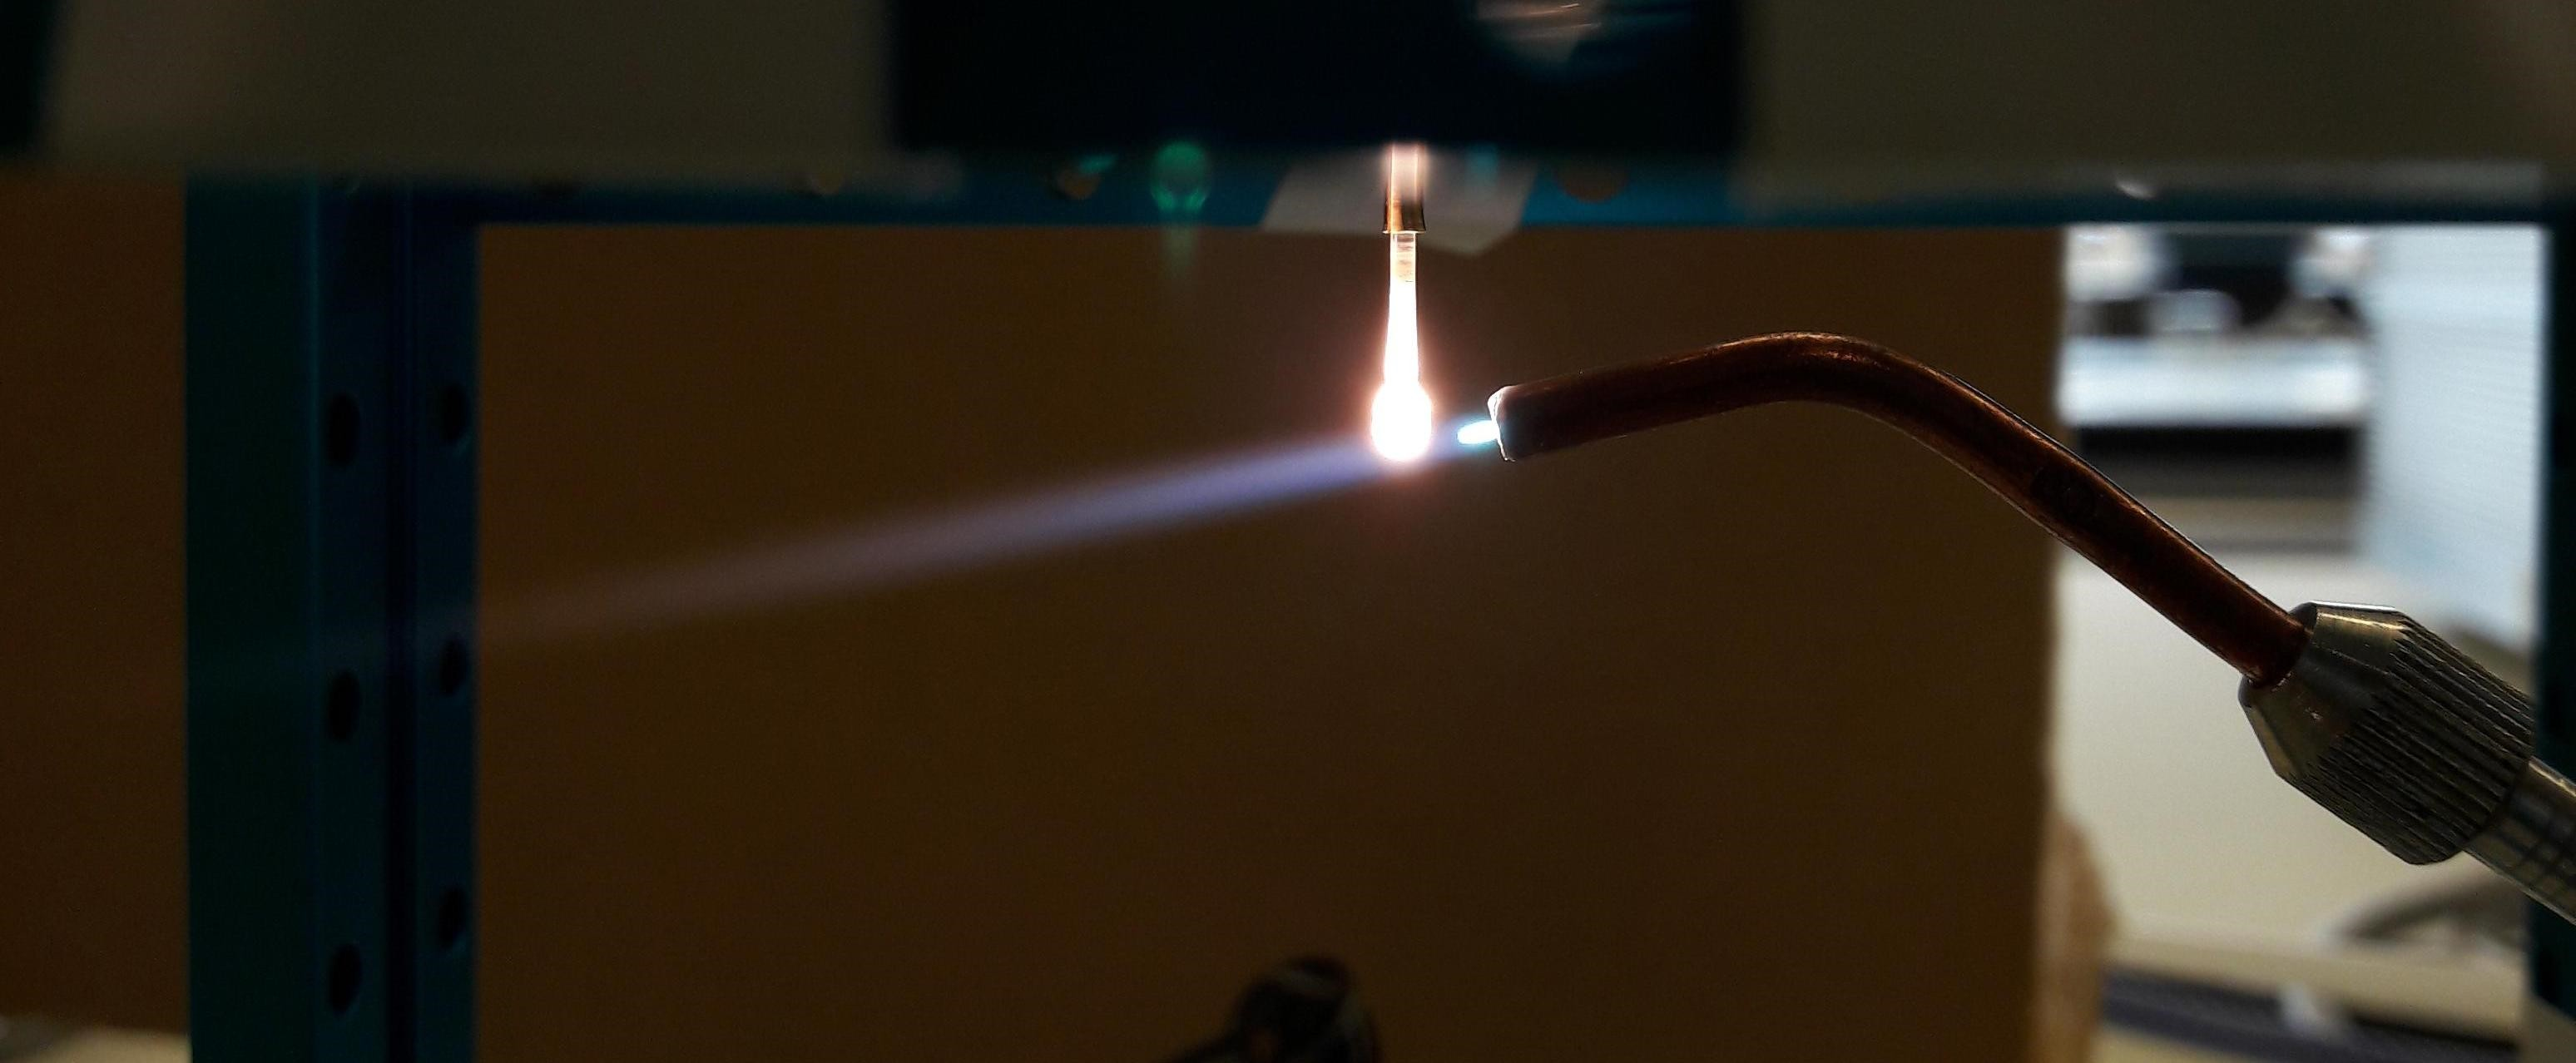
\includegraphics[scale=0.13]{source/melting}
	\caption{In this picture it can be seen how the rotating glass rod forms a drop which is spherical in the front. After cooling the surface is smooth [ref] and the stamp can be further processed.}
\end{figure}

\subsection{Measurement}\label{ChapMeasurement}
After the stamps have been fabricated their respective sphere radii have to be determined. The most frontal part of the glass stamp will imprint the spherical mirror shape into the polymer. This means that the radius of the front part of the stamp has to be known. For this purpose the stamps are fixed inside a quartz-dish and photographed with a microscope. From this image a software developed in python can determine the radius of the spherical region that will be used as the actual stamp.

\begin{figure}[H]
	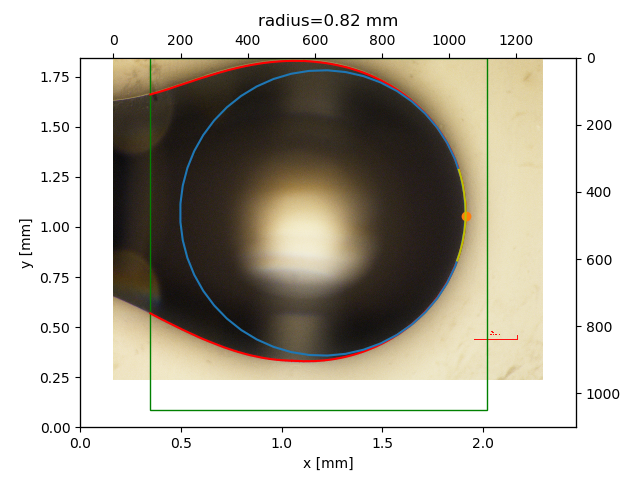
\includegraphics[scale=0.6]{source/radius_analysis}
	\caption{The software that is used for extracting the radius is developed in python. It is able to determine the orientation of a sample and uses this to predict which part of the stamp will be in contact with the polymer (marked yellow). The contact region is then used to extract the radius with at this position with the Ransac (Random sample consensus) [ref] algorithm.}
\end{figure}
From the radius we can then infer the dimensions of the actual mirror. First we need the beam waist radius in the focus so we can calculate the Rayleigh range. The wavefront radius is now fixed since the stamp is already fabricated and the cavity length we choose to be $500\si{\micro m}$ as discussed in \autoref{ChapCavityLength}. The following formula for the beam waist radius in the focus can be found by plugging \autoref{EqRayleighRange} into \autoref{EqWfRadius}:
\begin{equation}
	w_0(R, L)=\sqrt{\frac{\lambda}{\pi}}\left(L(R-L)\right)^{1/4}
\end{equation}
We know from our discussion regarding the the cavity length that the mirror diameter $D$ will be around $200\um$. Given that $R, L$ and $w_0$ are known we can use \autoref{BeamDiameter} to get a specific value for $D$. From this we can calculate the mirrors depth with simple, geometrical considerations:
\begin{equation}\label{EqH}
	h=R-\sqrt{R^2-\left(\frac{D}{2}\right)^2}
\end{equation}
The diameter of the mirrors surface that will actually be hit by the light can be calculated as follows:
\begin{equation}
	d_{\si{Beam}}=2R\cdot \arctan\left(\frac{w(L)}{R}\right)
\end{equation}
Where $L$ is the cavity length.
\begin{figure}[H]
	\includesvg[scale=0.8]{source/mirror}
	\caption{This sketch shows the different mirror dimensions quantities which can be estimated after the radius of the stamps has been determined.}
\end{figure}
The results of the measurements can be found in \autoref{table:CalcMirrorData}.

\subsection{Silanization}
As imprinting medium we use a polymer called OrmoComp (made by the German company Microresist) [ref]. This polymer is made for imprinting small details and curing it afterwards with UV-light. To improve the quality of the imprints it is important to use an anti-adhesive agent which prohibits the polymer from sticking to the stamp after it has been hardened. Anti-adhesive agents are chemical compounds which belong to the Silane group, hence the term \textit{silanization} [ref]. For our silanization we used a silane called \textit{1H,1H,2H,2H-perfluorooctyl-trichlorosilane} (usually shortened to \textit{F13-TCS}).
\begin{figure}[H]
	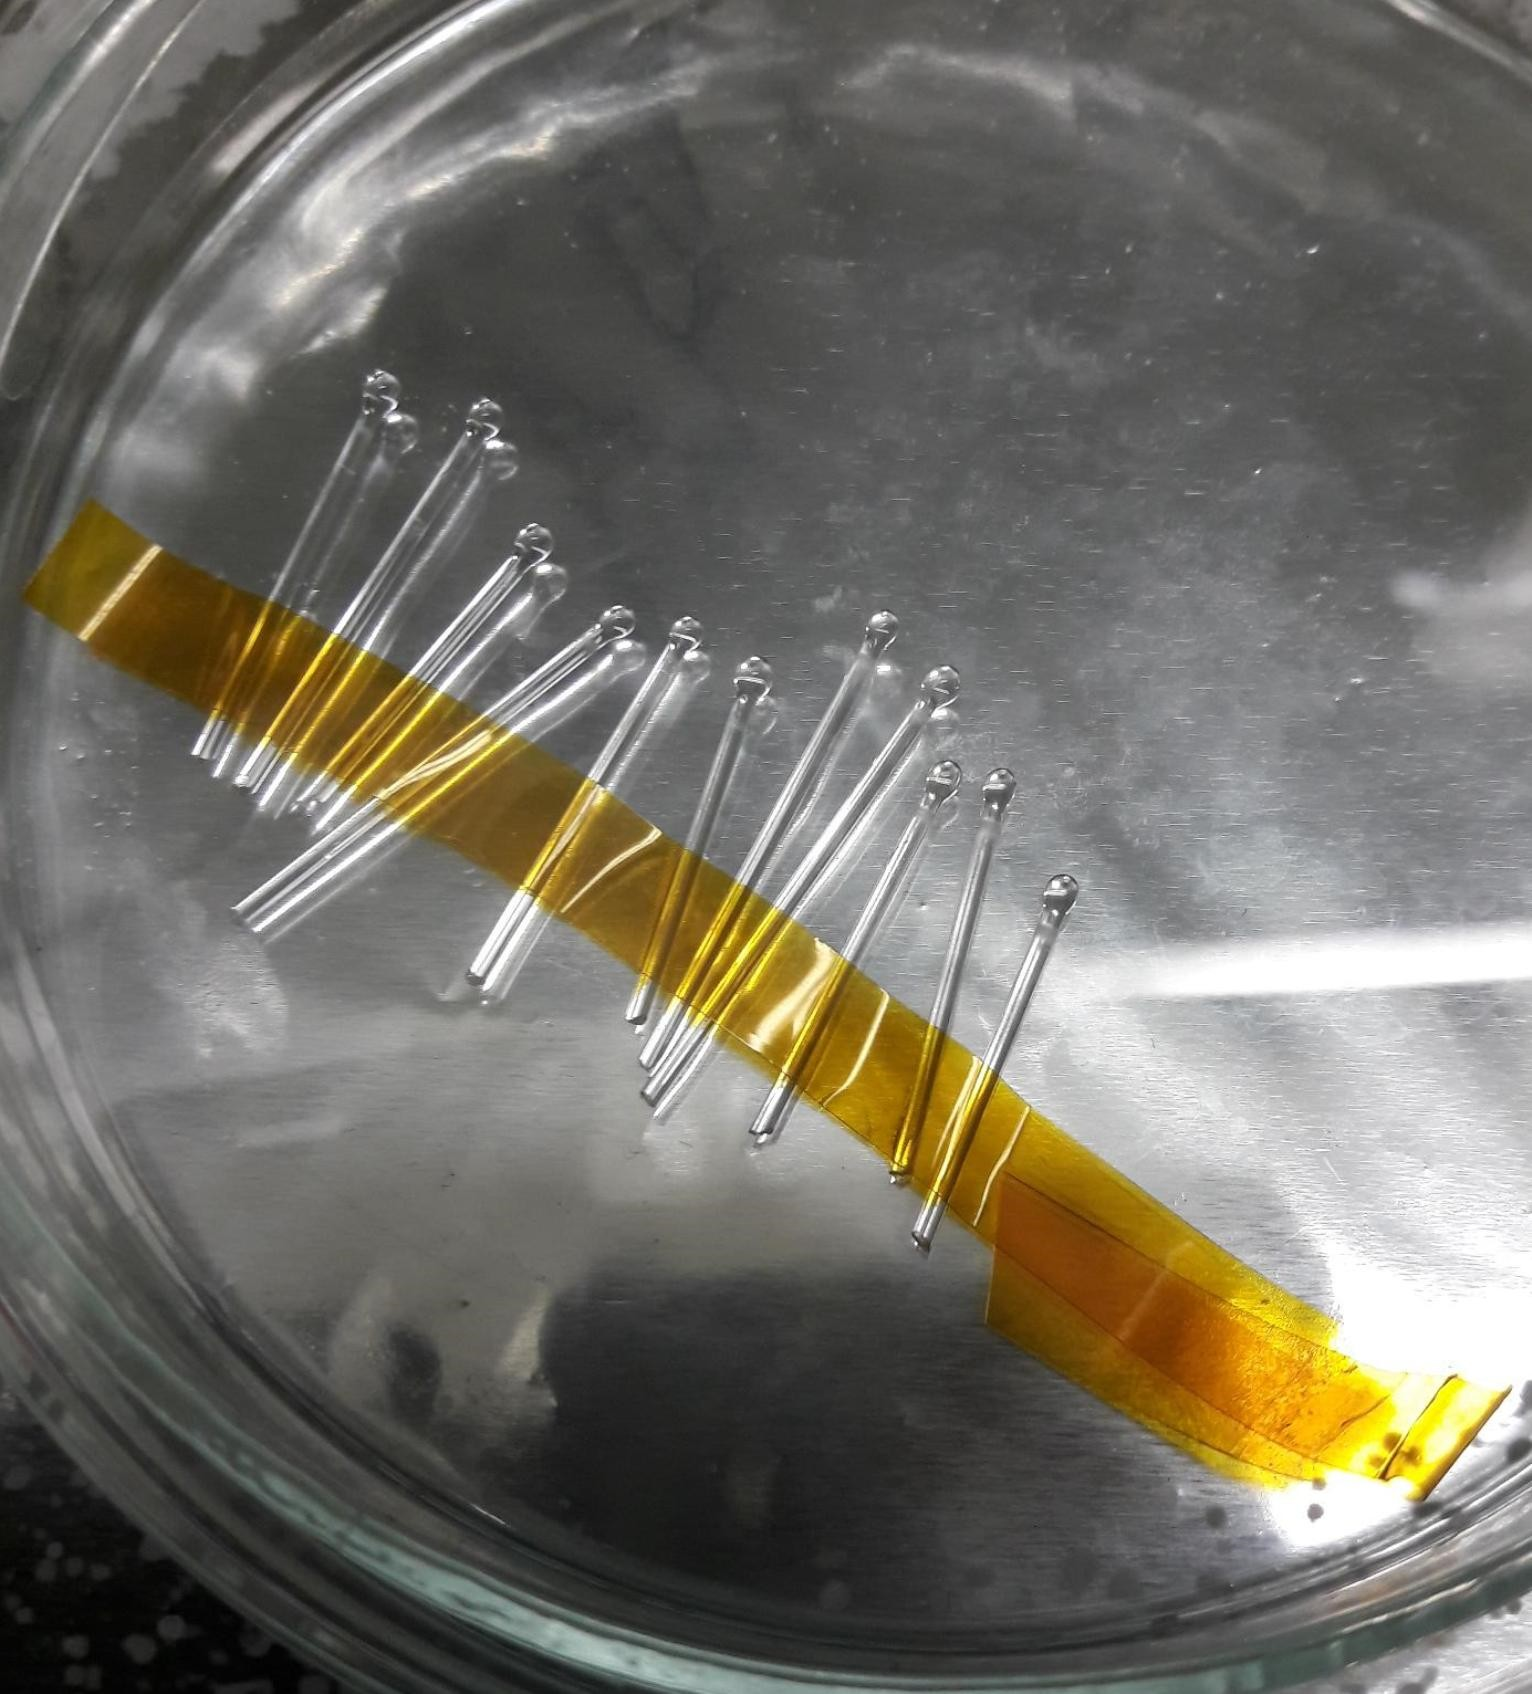
\includegraphics[scale=0.1]{source/stamps_taped}
	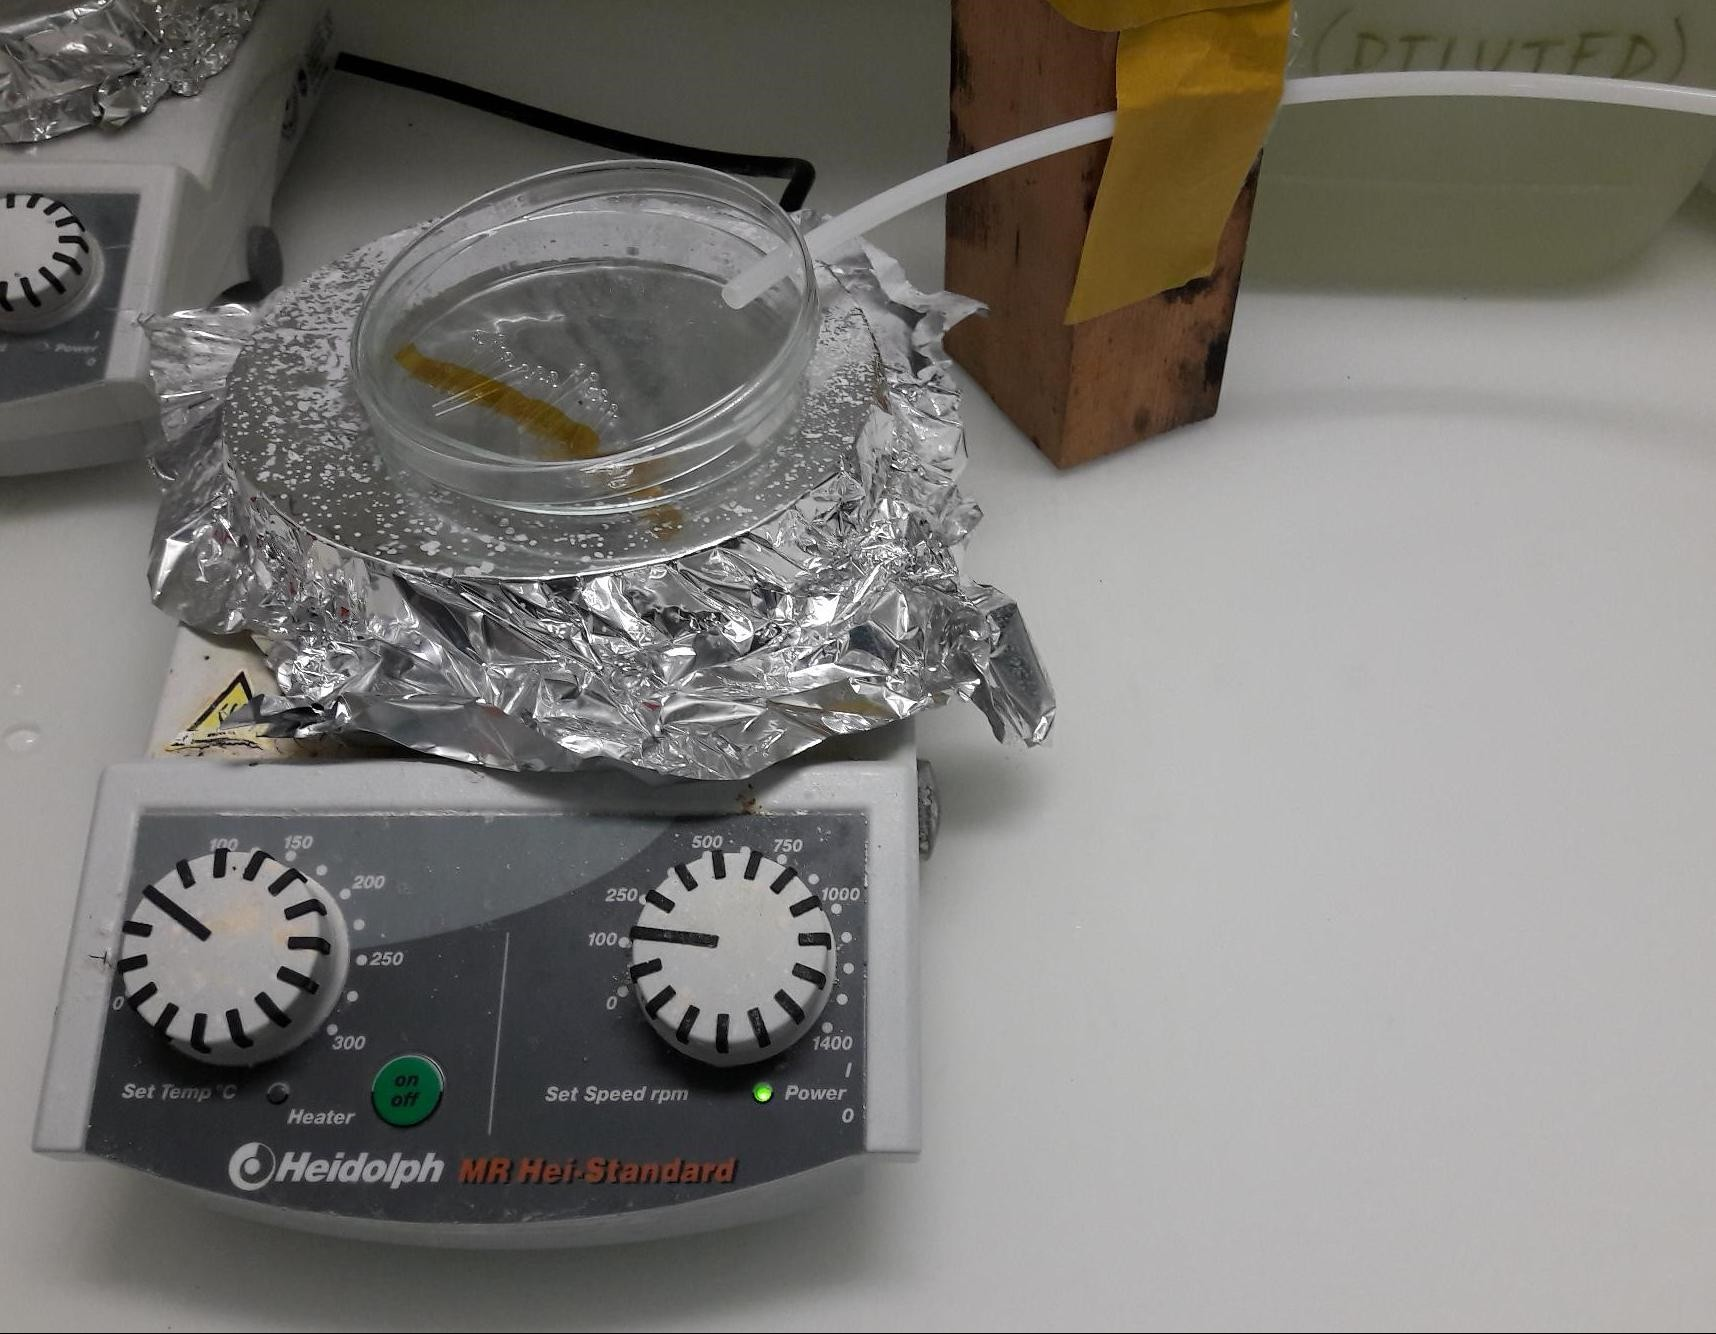
\includegraphics[scale=0.14]{source/silanization}
	\caption{Left: Stamps fixed at the bottom of the quartz dish. Right: Setup used for silanization.}
	\label{Fig:silanization}
\end{figure}
Since F13-TCS reacts strongly with water it is important that the moisture in the environment it kept at a minimum during the silanization process. To achieve this, we taped our stamps to the bottom of a quartz dish, put them onto a hot plate and flushed them with a weak but steady stream of nitrogen (see \autoref{Fig:silanization}). The entire process takes place under flow hood (model). This procedure continues for thirty minutes while the quartz dish is heated to $50\degrees$.\\
After thirty minutes, the nitrogen flow is removed and a small amount ($0.5-1.0\ul$) of the F13-TCS is put next to the stamps without touching them. At $50\degrees$ the silane will evaporate and ideally its molecules will bind to the surfaces of the stamps and build up an anit-adhesive monolayer [ref].\\
After an additional thirty minutes the hotplate is turned off. The quartz dish, remains closed and under the flow hood until it reaches room temperature.\\
There are process manuals which include a plasma treatment of the stamps upfront [ref]. In our process we have omitted this step since the stamps have been melted less than an hour prior to the silanization. The OH-groups that are exposed by the plasma treatment should also be present after melting. Tests that were conducted also confirmed that proper silanization can be achieved without prior plasma treatment of the stamps.

\subsection{Coverslip preparation}\label{ChapCoverslipPreparation}
The polymer which was described in the last section is located on a glass coverslip which serves as a base for the mirror. To add the polymer layer to the coverslip we follow a specific procedure.\\
First, we get the pre-cleaned coverslip from a beaker where it was stored in DI water. The coverslip is then dried and put into a plasma chamber ([device]). To enhance the adhesion of the polymer to the glass a treatment with oxygen plasma is applied over a duration of approximately two minutes. The next step is to use a spin-coating machine ([device]) to create an even layer of the polymer. This process takes place in a yellow room since the polymerization of the OrmoComp polymer which we are using, starts very quickly when exposed to UV-light sources. The spin-coating takes thirty seconds and takes place at a rotational speed of $3000\rpm$. The coated coverslip is then put onto a hotplate at $80\degrees$ and left there for two minutes. This concludes the coating and pre-baking, the polymer layer has now a thickness of $20-25\um$ [ref] and can be used for imprinting.

\subsection{Mirror imprinting}
With the stamps silanized and measured and a glass coverslip with a still fluid layer of polymer the next step is to imprint the mirror. From the measured radius of the stamp \autoref{EqH} is used to dictate how deep the mirror is supposed to be. During imprinting the stamp has to be lowered slowly onto the polymer layer until contact and then slowly pressed into the material until the desired depth is achieved. Details about variations in the imprinting mechanism will be discussed in \autoref{ChapMirrorFab}.\\
Once this is done the polymer has to be cured with UV light. The manufacturer recommends using a light source at $\lambda=365\nm$ and and exposure dose of $500$ to $1500 \mJcm$ [ref]. The UV source (US460 Lightpen) we used has $\lambda = 365\nm \pm 5\nm$ and a power of $30'000\Wm$ [ref]. This means that by exposing the mirror for one minute is effectively overexposing it. However, according to the process manual overexposing the polymer doesn't degrade the quality [ref].\\
After curing, the stamp is removed and the coverslip is put onto a hotplate for post backing. This takes place over ten minutes at $130\degrees$.

\subsection{Grinding}\label{ChapGrinding}
With the post backing procedure done, the mirrors would principally be ready for the measurement of their surface roughness under the atomic force microscope. Critically, a the mirrors during the development of this process turned out to be too wide and too deep for measurement. This also meant that they are ill dimensioned to be used in a microcavity.

\begin{figure}[H]
	\includesvg[scale=0.48]{source/grinding_sketch}
	\caption{Schematic depiction of the grinding process. In the top left sketch the desired mirror is drawn in red.}
	\label{fig:GrindSketch}
\end{figure}

To obtain the mirror dimensions necessary we used sandpaper to remove excess material. In \autoref{fig:GrindSketch} the grinding process is depicted. First, a cleaning fluid for optical components (First Contact) is applied over the whole surface. After six hours the fluid has dried and forms a protective layer for the mirror inside of the larger hole. The next step is to gradually remove the excess material with sandpaper. During this procedure the protective layer remains on the mirror and protects it from being damaged. For the first iteration a rougher sandpaper is used ($30\um$). Once the mirror starts to get smaller it is important to check frequently under the microscope how the diameter has changed (see \autoref{fig:GrindingMicroscope}). Switching to a smoother sandpaper ($3\um$) is important at a certain point.

\begin{figure}[H]
	\includegraphics[scale=0.5]{source/grinding/grinding}
	\caption{The microscope images show how the mirror diameter gets smaller during the grinding procedure. The protective layer can be seen over the entire sample in the top left and in the center region in the other images. The sandpaper leaves clearly visible marks wherever it removes material. (Images were digitally enhanced, microscope indicators were removed)}
	\label{fig:GrindingMicroscope}
\end{figure}
Getting the mirrors to a diameter $D=200\um$ is nearly impossible with this method. This coupled with the high risk of destroying the mirror itself makes this the most difficult step of the fabrication process. More problems and possible improvements will be discussed in \autoref{ChapProblems} and \autoref{ChapSolutions}.

\subsection{Cleaning}
The grinding procedure where the mirrors are dimensioned properly causes a lot of dirt on the mirror and the area around it. Furthermore, the dried optical cleaning liquid which was used as a protection layer is still inside the mirror. To remove the dirt and the protection layer residuals we apply the cleaning liquid again and wait for another six hours. After that, a pincer can be used to carefully peel of the newly dried layer, hopefully removing any dirt and residuals on the mirror. While not as difficult as the grinding procedure, cleaning still bares the risk of ripping the mirror from the rest of the material.

\begin{figure}[H]
	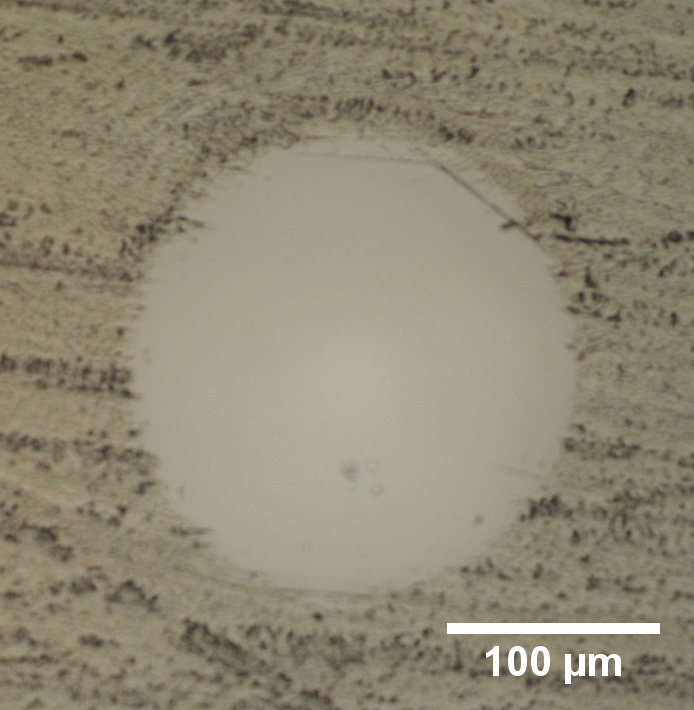
\includegraphics[scale=0.25]{source/cleaning_good_scale}
	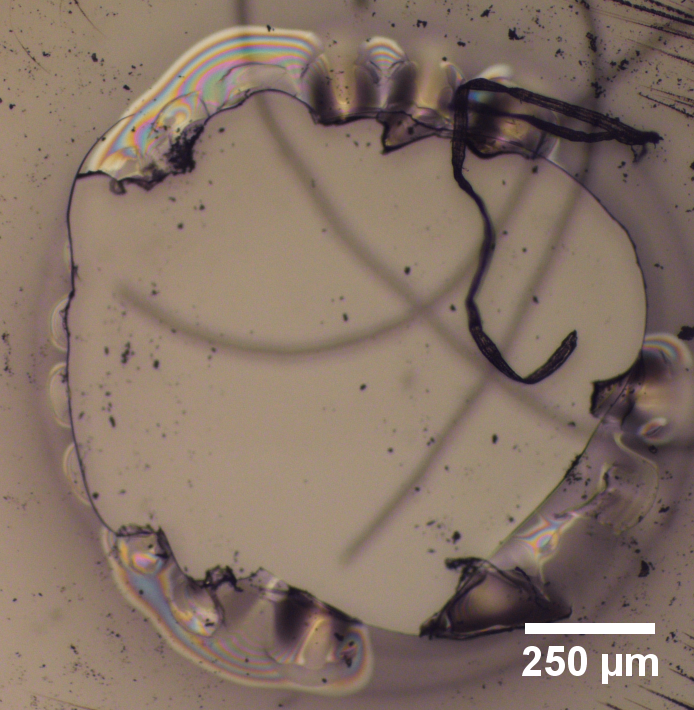
\includegraphics[scale=0.25]{source/cleaning_bad_scale}
	\caption{On the \textit{left} side a successfully cleaned mirror can be seen. Regardless of the success, scratch marks are clearly visible along the border of the mirror. On the \textit{right} side a site of a mirror, ripped out while cleaning can be seen.}
\end{figure}